\documentclass[full.tex]{subfiles}


% change this line
\graphicspath{ {assets/note5/} }
\newcommand{\notenum}{5}


\begin{document}
    \thispagestyle{firstpage}
    \vspace*{2\baselineskip}
    \section*{Cryptocurrency Mining: Proof-of-Work Consensus}
    
    Bitcoin mining is the process through which new bitcoins enter the network and is also what keeps the network healthy and resistant to malicious parties---an arms race that rewards those who invest the most into their hardware. But why do miners mine? What incentives do they have, and most importantly, is it profitable? In this section, we will explain in depth the design and mechanics behind Bitcoin mining, taking into account various mining incentives.
    
    \section*{Recap: What a Miner Does}
    
    \noindent In a nutshell, a Bitcoin miner accomplishes the following six tasks:
    
    \begin{enumerate}
        \item \textit{Download} the entire Bitcoin blockchain to store the entire transaction history.
        \item \textit{Verify} incoming transactions by checking signatures and confirming the existence of valid bitcoins.
        \item \textit{Create} a block using collected valid transactions.
        \item \textit{Find} a valid nonce to create a valid block header (this is the ``mining'' part).
        \item \textit{Hope} that your block is accepted by other nodes and not defeated by a competitor block.
        \item \textit{Profit!} Coinbase transacation rewards miners for their work.
    \end{enumerate}
    
    The Bitcoin miner maintains the Bitcoin network's health by creating valid blocks and participating honestly in the Proof-of-Work protocol. They ensure that (hopefully) only valid blocks make their way into the blockchain, receiving a bitcoin reward in exchange (also functioning as a mechanism through which new coin created in the Bitcoin network).
    
    \section*{Block Difficulty --- Analogy}
    
    Imagine a game in which you are blindfolded, throwing darts randomly at a dart board. (Say for simplicity that all your darts are guaranteed to land on the dartboard.) There is an equal likelihood of hitting any given point on the dartboard. If one of your darts lands within a certain radius $d$ from the center, then you get a reward. Throwing faster allows for more hits per second, granting a higher likelihood of any of your darts land within the target distance and a higher chance of winning the reward. 
    
    Now imagine competing with many other blindfolded individuals to hit the target first. The difficulty of hitting the target is inversely proportional to $d$. In other words, it's harder to hit a smaller target and easier to hit a larger one. To control how many rewards are distributed within a given period of time, $d$ changes depending on the average time taken to hit the target. This way, if people get better at throwing darts, then $d$ gets smaller, and vice versa.
    
    \section*{Block Difficulty --- Puzzle Prerequisites}
    
    Instead of blindly throwing darts at a dartboard, mining in Bitcoin involves solving a \textbf{hash puzzle} that results in a valid block. Miners race each other to find a nonce that makes the following inequality true:
    $$H\big(nonce~||~H(previous~block~header)~||~Merkle~root\big)~<~target$$
    
    \noindent Hash puzzles must meet a few significant requirements:
    \begin{itemize}
        \item Computational difficulty. If finding the proof-of-work required little work, then reaching consensus would be difficult (See Note 4). This is why in the analogy, we blindfolded the dart-throwers. 
        \item Variable cost. This allows for adjustments as the global hash power changes, to let the puzzle difficulty change alongside it. In the analogy, the target size changes with $d$.
        \item Easily verifiable. There should not be a need for a central authority to verify nonce validity. Every miner simply rehashes the nonce and other relevant information to verify validity. In the dart analogy, darts stick to the dartboard, so to verify, others simply have to take their blindfolds off to verify.
    \end{itemize}
    
    \section*{Block Difficulty --- Adjustment}
    
    \noindent The following is the equation to adjust the \textbf{difficulty} of the hash puzzle used in Bitcoin:
    $$\mathit{difficulty}~=~\mathit{difficulty~*~two\_weeks~/~time\_to\_mine\_prev\_2016\_blocks}$$
    
    \noindent We use the ratio between two weeks and the time to mine 2016 blocks because the target block time is 10 minutes:
    $$\mathit{2016~blocks~*~10~\frac{min}{block}=20160~min=2~weeks}$$
    
    If the time to mine 2016 blocks is greater than two weeks, then the hash puzzle is too hard. The ratio is less than 1, so the difficulty scales down. If the time to mine 2016 blocks is less than two weeks, then the hash puzzle is too easy. The ratio is greater than 1, so the difficulty scales up. The block difficulty is always inversely proportional to the time required to mine the previous 2016 blocks.
    
    \section*{How to Profit From Mining}
    
    \noindent For the Bitcoin miner, the following equations are true.
    \begin{align*}
        \begin{split}
            \mathit{MINING\_REWARD}~&=~\mathit{BLOCK\_REWARD~+~TX\_FEES} \\
            \mathit{MINING\_COST}~&=~\mathit{HARDWARE\_COST~+~OPERATING\_COSTS}
        \end{split}
    \end{align*}
    
    \noindent If mining rewards exceed mining costs, then a Bitcoin miner will profit. In the next sections, we will analyze each of the components in the above equations.
    
    \section*{Block Reward}
    
    A Bitcoin miner receives bitcoins for producing valid blocks. As of July $23^{rd}$ 2017, the block reward is 12.5 BTC per block. Potential profit incentivizes honest behavior. The Bitcoin protocol requires finding the proof-of-work first, broadcasting the associated block, and awaiting confirmation to receive a \textbf{block reward}. In a block, the miner must include a special transaction to themselves, known as the \textbf{coinbase transaction}. The block reward halves every 210,000 blocks to cap the total number of bitcoins that will ever be produced. In other words, Bitcoin is a \textbf{deflationary} currency, topping off in 2140 at 21,000,000 BTC (the supply cap).
    
    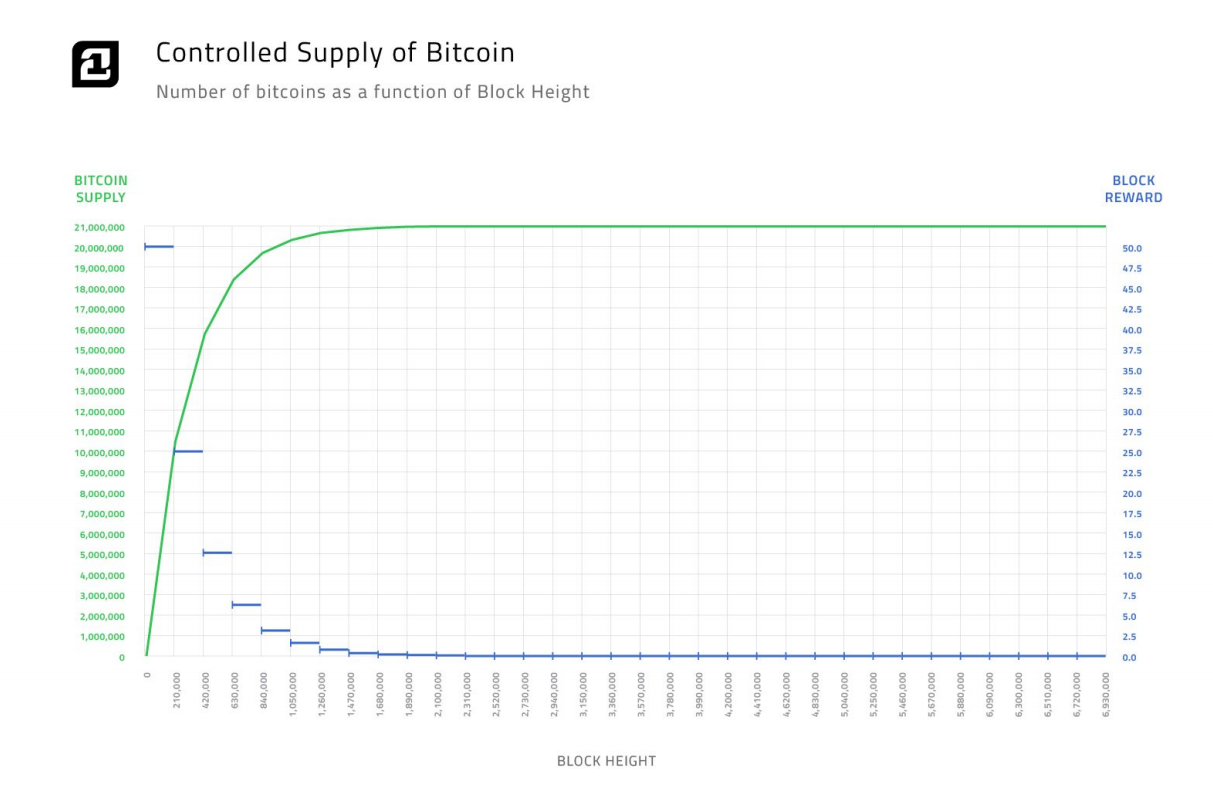
\includegraphics[scale=0.33]{supply_cap}
    \section*{Transaction Fees}
    
    The creator of a transaction sets the transaction fee, a voluntary but practically necessary incentivize miners into prioritizing your transaction. In practice, a higher transaction fee leads to a faster confirmation time. Transaction fees provide extra income to miners on top of the block reward, increasingly important as block rewards diminish. When the block reward becomes 0, transaction fees will become the sole source of revenue for miners. To calculate transaction fees, simply subtract the output from the input amounts for the transaction. The difference implicitly becomes the transaction fee. 
    \begin{center}
    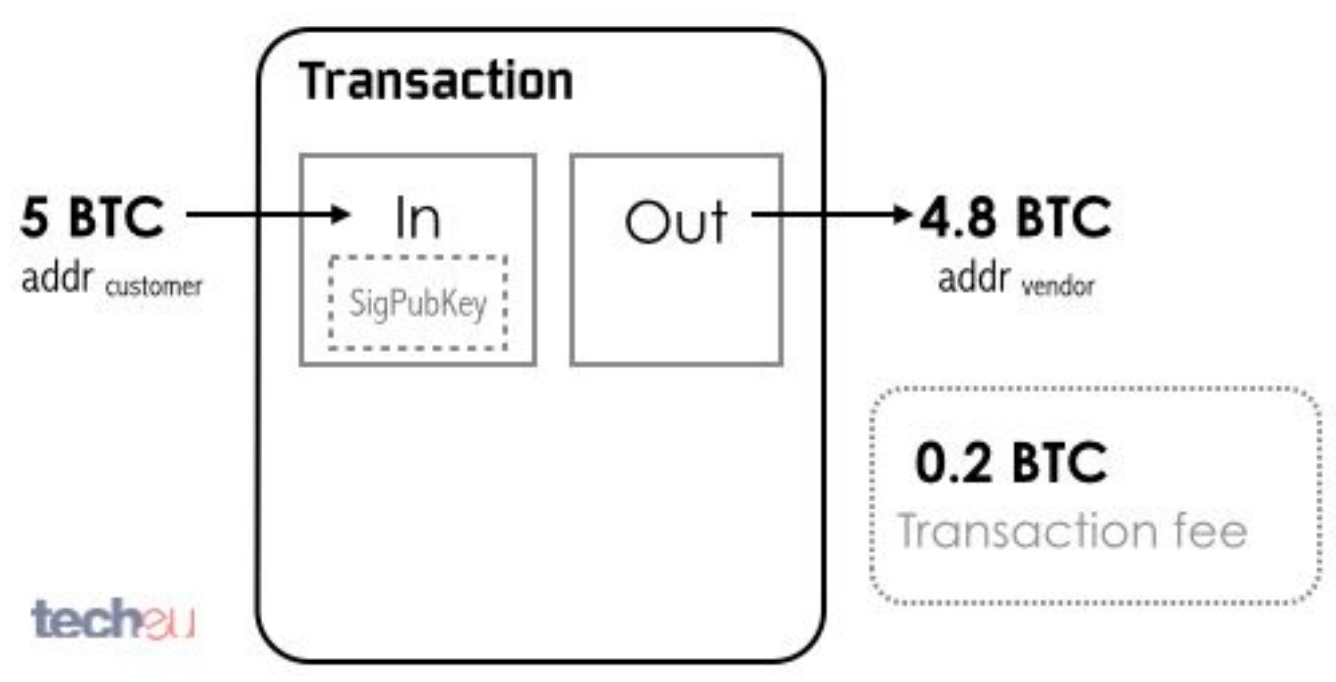
\includegraphics[scale=0.22]{transaction_fee}
    \end{center}
    
    In the figure above, the input is 5.0 BTC and the output is 4.8 BTC. The creator of this bitcoin transaction has included an implicit transaction fee of 0.2 BTC that is to be collected by the miner who includes this transaction in the block that is confirmed by the rest of the network.

    \section*{Hardware Cost}
    
    Bitcoin mining began on CPUs. As the block difficulty increased, mining efforts shifted dramatically: first to GPUs, then to FPGAs, and finally to ASICs. (Keep in mind that hardware costs are a one-time expense, unlike everything else we have mentioned.)
    
    As commonly used CPUs began to get too slow for the block difficulty, GPU mining began to gain popularity. GPUs are an order of magnitude more effective for hashing than CPUs. However, with more power comes more expense: a larger consumption of energy and higher production of heat. GPU mining was most common around 2012, but as of now is not viable for mining Bitcoin. (GPU mining is viable for Zcash, Ethereum, and some other cryptocurrencies on the other hand.) GPU mining brought two main disadvantages:
    
    \begin{enumerate}
        \item GPUs have many components (like floating point units) not applicable to Bitcoin mining.
        \item GPUs are not meant to be run in ``farms'' side by side.
    \end{enumerate}
    
    The disadvantages of GPU mining made clear the need to switch to mining specific hardware.
    
    \textbf{FPGAs (Field Programmable Gate Arrays)} were the result of early efforts to develop Bitcoin-specific hardware without losing all hardware customizability, a trade-off between dedicated, specialized hardware and general purpose functionality. If Bitcoin failed, SHA-256 specific hardware would be worthless, but general purpose hardware would still be useful. However, if Bitcoin thrives, specialized hardware for churning out SHA-256 calculations would generate higher profit than generalized hardware. Hence, compromise.
    
    As Bitcoin rose in popularity, general purpose hardware was dropped altogether by many to create the first \textbf{ASICs (Application-Specific Integrated Circuits)}. ASICs for Bitcoin do nothing but SHA-256, but they do it better than any other hardware. ASICs, a diverse breed, come with various tradeoffs,  one of which is between base cost and electricity usage, depending on how efficiently it uses energy. Another is device size and hashrate, as larger devices take up more space and use more electricity but have a higher overall hashrate. Also, manufacturing and purchasing ASICs takes large upfront capital, which induces centralization---a tradeoff with Bitcoin's core decentralized philosophy. Currently, the Antminer 29 holds the title of ``Most Powerful ASIC," maxing out at 14 TH/s, purchasable for the steep price of 3000 USD.
    
    \section*{Operating Costs}
    
     \noindent Bitcoin mining operating costs fall into into three primary categories:
     \begin{itemize}
        \item \textbf{Embodied energy:} to produce mining hardware. 
        \item \textbf{Electricity:} to power the hardware. 
        \item \textbf{Cooling:} to maintain hardware health. 
    \end{itemize}
    
    All energy turns into heat, dissipating into the air without serving any further purpose. Over the years, initiatives arose to reuse heat generated by operating mining hardware. The ``data furnace'' idea involves using mining hardware as a heater. An average household could mine bitcoins during the winter to heat up their home while making money on the side.
    
    \section*{ASIC-Resistance --- Pros and Cons}
    
    Calls for \textbf{ASIC-resistance} developed based on arguments that mining should not be facilitated with specialized hardware, that there should be no significant benefit when running a mining algorithm in an ASIC as compared a CPU. ASICs are currently the only viable option for mining bitcoins, dominating the Bitcoin network and suppressing regular people. An ASIC-resistant Bitcoin means increased democracy and decentralization, as ASIC farms would have less power over the average CPU miner.
    
    However, there is also a strong case against ASIC-resistance. ASICs can only solve the Bitcoin hash puzzle, rendered to useless electricity-gobbling hardware in the event of a Bitcoin crash. (Attackers could rent general computing resources, however, resulting in no wasted investment---what then? Exercise for the reader.) Investment into expensive ASIC hardware becomes worthless without a puzzle to solve, discouraging attacks on the Bitcoin network. By that rationale, ASICs promote network security.
    
    \section*{ASIC-Resistance --- Memory-Hard Puzzle}
    
    Movements to make Bitcoin ASIC-resistant stirred consideration of            \textbf{memory-hard puzzles}, requiring large amounts of memory rather than computational power to solve. In other words, these puzzles are \textbf{memory-bound}, meaning that memory bottlenecks computation time. Memory-hard puzzles would viably deter ASICs and effectively make Bitcoin ASIC-resistant. ASICs are optimized to perform a specific algorithm while regular CPUs are not, and since optimization of this algorithm (in our case, a hash function) is not the limiting agent, ASICs would not give some miners more power if memory is the limiting agent, not computational optimization. Memory performance increases more slowly than computational power. The cost of solving a puzzle also decreases more slowly, all valid considerations in the ASIC-resistance debate among Bitcoin users.
    
    \section*{Scrypt}
    
    \textbf{Scrypt} (pronounced ``ess crypt'' and lowercase by default) is an algorithm used by Litecoin and Dogecoin for enforcing a memory-hard Proof-of-Work puzzle. Designed for hashing passwords and preventing brute force attacks, scrypt demands high memory space, making the size and cost of potential specialized hardware much more expensive than those for other algorithms. 
    
    \noindent Scrypt's two main steps:
    \begin{enumerate}
        \item A user must first fill a buffer with interdependent (pseudorandom) data. 
        \item The user accesses the memory buffer in a pseudorandom way until a correct hash is found.
    \end{enumerate}
    As a drawback, scrypt requires equal memory to verify, contrary to hash puzzle requirements. In addition, against scrypt's entire meaning for existing as a cryptocurrency hash puzzle, scrypt ASICs have been developed, killing the ASIC-resistance claim.
    
    \section*{ASIC-Resistance --- Other Approaches}
    
    Memory-hard algorithms such as scrypt do not provide real-world ASIC-resistance. Initiatives using technologies such as \textbf{x11} and \textbf{x13} hash function chaining have been proposed and implemented. Dash uses x11, which chains together 11 different hash functions. Designing ASICs for x11 and x13 systems are significantly harder than designing ASICs for SHA-256 but but are not impossible, it has been done.
    
    There is also the idea of periodically switching a mining puzzle. For example, a cryptocurrency system could go from SHA-1 to SHA-3 to Scrypt every 6 months. However, this solution is easy to work around for anyone who knows the rotation schedule. Naturally, this solution has also not been implemented. In short, ASIC-resistance seems like an impossible goal. As Mike Hearn, Bitcoin Core developer, famously stated: ``There's really no such thing as an ASIC-resistant algorithm."
    
    \section*{Proof-of-Useful-Work}
    
    Instead of having the world's most powerful network of assigned computers incrementing and recalculating one math problem, why not have a massive collective of computational power do some useful work? \textbf{Proof-of-useful-work} aims to repurpose the computational power of a Proof-of-Work cryptocurrency network to solve important problems. Historically, long-term public research projects produced great findings, encouraged by Proof-of-useful-work's attempts to repurpose mining compute power to aid through:
    
    \begin{itemize}
        \item Searching for large primes --- Great Internet Mersenne Prime Search, which found the ``largest prime number'' to date ($2^{57885161} - 1$) twelve straight times.
        \item Finding aliens --- SETI@home, which is the largest project to date, with over 5 million participants.
        \item Simulating proteins at the atomic level --- Folding@home, which has the greatest computing capacity of any volunteer computing project, and has produced more than 118 scientific papers. 
        \item Securing cryptography --- distributed.net, which was the first successful public brute-force of a 64-bit cryptographic key.
        \item Generating predictive climate models 
        \item Producing solar power (Solarcoin distributes coin to those who can produce solar power).
    \end{itemize}
    
    As good as Proof-of-useful-work sounds, design restrictions prohibit its consideration for cryptocurrencies and blockchain. Many distributed computing problems are unsuitable for Proof-of-Work, as a fixed amount of data will lead to trouble. For example, contributers to SETI@Home could run out of raw radio telescope data, leaving no problem to solve. Distributed computing problems lack an inexhaustible puzzle space, rendering them unfeasible. Second, potential solutions to these computing problems are not equally likely, so there is a lack of equiprobably solution space. Third, we must not rely on a central entity to delegate tasks, otherwise we fail to reach the requirement of decentralized and algorithmically generated problems. Thus, Proof-of-useful-work is unviable.
    
    \section*{Proof-of-Storage --- Permacoin}
    
    Instead of distributing work across a network, one idea involves distributing large files. In \textbf{Proof-of-Storage}, specifically the Permacoin implementation, a large public file in need of replication is split to be contained by several anonymous peers. An example of such a file would be experimental data from the Large Hadron Collider, several hundred petabytes of data. Such a file is stored in blocks, in a Merkle tree upon which the network agrees, then distributed to miners. Each stores a subset of these blocks, $T$, based off their public key to ensure that everyone agrees on who is responsible for what. They then continuously hash consensus information with a nonce to pick blocks in their stored subset and find a valid nonce such that its hash with all block headers is less than some target. Each server can query a given index, which returns a block header for the public data. One drawback to Proof-of-storage is that it is hard to find a large enough file to subsection to the network's nodes. If such a file is found, it would be difficult to change the block difficulty or to modify the file.
    
    \section*{Merge Mining}
    
    Consider the potential vulnerabilities of a new altcoin in the current market. Lack of hash power in the altcoin's network means lack of security. An individual can easily amass enough hash power to attack the small network. However, mining is exclusive by default; what is the incentive to mine and attack an altcoin if you can instead make profit on the Bitcoin blockchain? Despite this lack of coin/cash incentive, cases of ``altcoin infanticide'' aren't new. Altcoins with their minimally connected networks are vulnerable to attacks from miners from larger coins (Bitcoin) with much more hash power than that of the entire altcoin. In 2012, Eligius mining pool attacked CoiledCoin, reversing multiple days' worth of transactions.
    
    The solution to the problem of altcoins being too weak is to implement \textbf{merge mining}. Merge mining involves creating blocks with transactions from both Bitcoin and an altcoin. The problem would be how to incentivize miners to include altcoin transactions in Bitcoin. Solving this requires including a Merkle root of altcoin transactions in Bitcoin's coinbase parameter. Bitcoin miners could then reap both Bitcoin and altcoin rewards. This would result in no additional cost and no profit loss at all. \\
     
   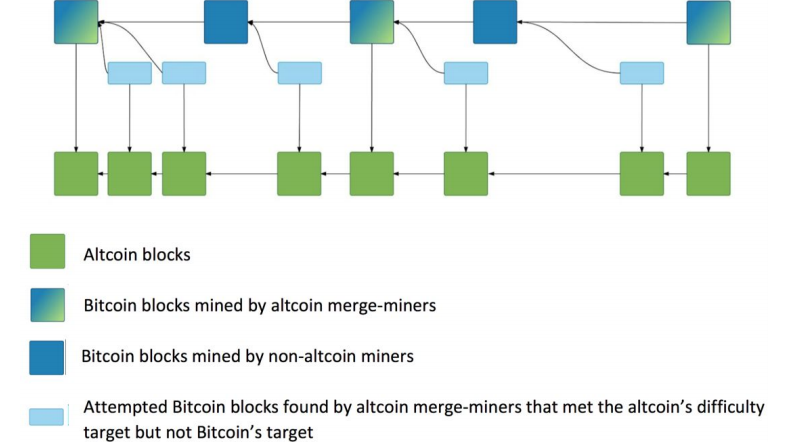
\includegraphics[scale=0.5]{merge} \\
   
    
    
    % BEGIN KEY TERMS
    \newpage
    \thispagestyle{firstpage}
    \vspace*{2\baselineskip}
    \section*{Key Terms}
    \noindent A collection of terms mentioned in the note which may or may not have been described. Look to external sources for deeper understanding of any non-crypto/blockchain terms.
    \begin{enumerate}
        % edit within here
        \item \textbf{VOCAB WORD} --- Definition. % format
    \end{enumerate}
    % END KEY TERMS
\end{document}